\documentclass[letterpaper,11pt,leqno]{article}
\usepackage{paper}
\usepackage{float}
\usepackage{graphicx}
\usepackage{hyperref}
\usepackage{subcaption}
\usepackage{geometry}
\geometry{margin=1in}

\bibliographystyle{paper}

\usepackage{booktabs}
\usepackage{multirow}
\usepackage{tabularx}
\usepackage{tikz}
\usepackage{colortbl}
\usepackage{xcolor}
\usetikzlibrary{positioning, fit, arrows.meta, shapes.geometric, calc, backgrounds,
                shadows, decorations.pathreplacing}
\hypersetup{pdftitle={Prompt tuning Ideas on top of LoRA}}

\newcommand{\bib}{paper.bib}

% Custom colors
\definecolor{bestgreen}{HTML}{C8E6C9}
\definecolor{worstred}{HTML}{FFCDD2}
\definecolor{midyellow}{HTML}{FFF9C4}
\definecolor{sectionblue}{HTML}{E3F2FD}
\definecolor{run1blue}{HTML}{4C72B0}
\definecolor{run2orange}{HTML}{DD8452}
\definecolor{run3green}{HTML}{55A868}
\definecolor{run4red}{HTML}{C44E52}
\definecolor{run5purple}{HTML}{8172B3}
\definecolor{run6pink}{HTML}{E91E63}
\definecolor{run7teal}{HTML}{00897B}
\definecolor{run8rust}{HTML}{D84315}
\definecolor{run9ocean}{HTML}{0288D1}
\definecolor{run10violet}{HTML}{6A1B9A}

\begin{document}

\title{Prompt tuning Ideas on top of LoRA}
\author{Mohammad Yavari}
\date{August 2026 \\[0.5em] \small Repository: \url{https://github.com/myavarih/CLIP-LoRA}}

\begin{titlepage}
\maketitle
\end{titlepage}

\tableofcontents
\newpage

% ============================================================================
\section{Why?}
% ============================================================================

In earlier experiments, plain LoRA was observed to place textual prompt representations very close to each other in PCA and t-SNE spaces. In addition, good natural names or clear descriptive phrases are not readily available for our target classes. Therefore, it was thought that learning prompts for the text encoder might improve performance. Two directions were tested: replacing LoRA in the text encoder with prompt tuning approaches, and adding prompt tuning directly on top of LoRA for the text encoder.

Furthermore, our classes naturally group into clusters of ordinal grades (such as \textit{Brown Momtaz} and \textit{Brown Plus}). A well-behaved model should ideally confuse \textit{Brown Momtaz} with \textit{Brown Plus} if a mistake is made, rather than confusing it with a completely different category such as \textit{Lux}! To address this, a table of custom losses (a cost matrix) aligned with our specific classes was introduced.

Another idea tested was to use PromptSRC to dial down catastrophic forgetting.

Here is a summary of the runs tested (note that all runs were evaluated on only a single seed, but meaningful conclusions can still be drawn given the substantial performance differences):

\begin{table}[H]
\centering
\begin{tabularx}{\textwidth}{l l X}
\toprule
\textbf{Run} & \textbf{Name} & \textbf{Key Addition} \\
\midrule
Run 1 & CoOp-LoRA Baseline          & CoOp text prompts + Vision LoRA ($r{=}2$, $\alpha{=}1.0$) \\
Run 2 & + Residual Class Tokens     & Learnable $\Delta w_c$ per class \\
Run 3 & + Ordinal Cost Loss         & $\mathcal{L}_\mathrm{CE} + \lambda\,\mathcal{L}_\mathrm{ord}$ \\
Run 4 & + PromptSRC Regularisation  & KL self-consistency + cosine anchors \\
Run 5 & + Full Unified Method       & All components combined: $\Delta w_c + \mathcal{L}_\mathrm{ord} + \mathcal{L}_\mathrm{src}$ \\
Run 6 & Residual-Template LoRA (RT-LoRA) & Natural template + Class/Template deltas + Dual LoRA + Ordinal Loss \\
Run 7 & CoOp-CSC + Vision LoRA      & Class-Specific Context ($N_\text{cls} \times M$ tokens) + Vision LoRA + Ordinal Loss \\
Run 8 & CoOp-CSC + Dual LoRA        & Class-Specific Context ($N_\text{cls} \times M$ tokens) + Dual (Vision \& Text) LoRA + Ordinal Loss \\
Run 9 & Staged CSC (100it) + Vision LoRA & Class-Specific Context trained for 100 iters then frozen + Vision LoRA + Ordinal Loss \\
Run 10 & Staged CSC (100it) + Dual LoRA   & Class-Specific Context trained for 100 iters then frozen + Dual LoRA + Ordinal Loss \\
\bottomrule
\end{tabularx}
\end{table}

All runs use the Walnut dataset (6 classes, graded quality scale), ViT-B/16
backbone, seed~1, and the shot grid $k \in \{1, 2, 4, 8, 16, 32\}$.

% ──────────────────────────────────────────────────────────────────────────────
\subsection{Architecture Diagrams}
% ──────────────────────────────────────────────────────────────────────────────

Figure~\ref{fig:coop_lora_arch} illustrates the shared hybrid architecture combining $M{=}4$ learnable context tokens with vision LoRA adaptation, upon which the ablation variants (Runs~2--5) are constructed.

\begin{figure}[H]
\centering
\begin{tikzpicture}[
    frozen/.style={rectangle, rounded corners=5pt, fill=blue!10, draw=blue!40,
                   minimum width=3.8cm, minimum height=0.7cm, align=center,
                   font=\small, line width=0.5pt},
    trainable/.style={rectangle, rounded corners=5pt, fill=orange!15, draw=orange!50,
                      minimum width=3.8cm, minimum height=0.7cm, align=center,
                      font=\small, line width=0.5pt},
    extra/.style={rectangle, rounded corners=5pt, fill=green!12, draw=green!40,
                  minimum width=3.8cm, minimum height=0.7cm, align=center,
                  font=\small, line width=0.5pt},
    arr/.style={-{Stealth[length=4pt]}, gray!60, line width=0.5pt},
]

% Vision side (left column)
\node[font=\small\bfseries] (vtitle) at (-3.8, 8.2) {Vision Encoder};
\node[frozen]  (vpatch)  at (-3.8, 7.5) {Patch Embed};
\node[frozen]  (vtrans)  at (-3.8, 6.4) {12× ViT Blocks};
\node[trainable] (vlora) at (-3.8, 5.3) {LoRA on Q, K, V};
\node[frozen]  (vln)     at (-3.8, 4.2) {LayerNorm + Proj};
\node[font=\scriptsize\bfseries] (vfeat) at (-3.8, 3.5) {Image Features $\mathbf{I}$};
\draw[arr] (vpatch) -- (vtrans);
\draw[arr] (vtrans) -- (vlora);
\draw[arr] (vlora)  -- (vln);
\draw[arr] (vln)    -- (vfeat);

% Text side (right column)
\node[font=\small\bfseries] (ttitle) at (3.8, 8.2) {Text Encoder};
\node[trainable] (tctx)  at (3.8, 7.5) {Learnable Context $[V_1 \ldots V_4]$};
\node[frozen]   (ttrans) at (3.8, 6.4) {12× Transformer Blocks};
\node[frozen]   (tln)    at (3.8, 5.3) {LayerNorm + Proj};
\node[font=\scriptsize\bfseries] (tfeat) at (3.8, 4.2) {Text Features $\mathbf{T}_c$};
\draw[arr] (tctx)  -- (ttrans);
\draw[arr] (ttrans)-- (tln);
\draw[arr] (tln)   -- (tfeat);

% Class token delta (Run 2 & 5 extra)
\node[extra] (delta) at (3.8, 3.0) {$\Delta w_c$ (Runs 2 \& 5)};
\draw[arr, dashed, green!50] (tfeat) -- (delta);

% Similarity
\node[frozen] (sim) at (0, 2.0) {Cosine Similarity $\rightarrow$ Softmax};
\draw[arr] (vfeat) -- (sim);
\draw[arr] (tfeat) -- (sim);
\draw[arr] (delta)  -- (sim);
\node[font=\scriptsize\bfseries] at (0, 1.3) {Predicted Probabilities};

% Legend
\begin{scope}[shift={(-5, 0.5)}]
    \node[rectangle, fill=blue!10, draw=blue!40, minimum width=0.6cm, minimum height=0.3cm] at (0,0) {};
    \node[font=\scriptsize, anchor=west] at (0.4, 0) {Frozen};
    \node[rectangle, fill=orange!15, draw=orange!50, minimum width=0.6cm, minimum height=0.3cm] at (0,-0.5) {};
    \node[font=\scriptsize, anchor=west] at (0.4, -0.5) {Trainable (all runs)};
    \node[rectangle, fill=green!12, draw=green!40, minimum width=0.6cm, minimum height=0.3cm] at (0,-1.0) {};
    \node[font=\scriptsize, anchor=west] at (0.4, -1.0) {Runs 2 \& 5};
\end{scope}

\end{tikzpicture}
\caption{Shared CoOp-LoRA architecture.  Orange = trainable in all runs.
Green $\Delta w_c$ is the residual class-token offset added in Runs~2 and~5.
The vision LoRA adapters sit inside each of the 12 ViT blocks.}
\label{fig:coop_lora_arch}
\end{figure}

% ──────────────────────────────────────────────────────────────────────────────
\subsection{What Each Run Tests}
% ──────────────────────────────────────────────────────────────────────────────

\paragraph{Run 1 --- CoOp-LoRA Baseline.}
Replaces the fixed hand-crafted prompt \texttt{"a photo of a [class]"} with
four learnable continuous context vectors $[V_1, V_2, V_3, V_4]$ placed before
the class token.  The class token embeddings themselves are frozen.  The vision
encoder is adapted by LoRA ($r{=}2$, $\alpha{=}1.0$) on the Q, K, V projections.
Loss is standard cross-entropy.

\paragraph{Run 2 --- Residual Class Tokens.}
Adds a per-class learnable offset $\Delta w_c$ initialised at zero, so the
effective class embedding becomes $\hat{w}_c = w_c + \Delta w_c$.  This directly
compensates for CLIP's tokeniser fragmenting domain-specific Persian
transliterations (e.g.\ \textit{siah goshti}, \textit{momtaz}) into
semantically noisy sub-tokens.

\paragraph{Run 3 --- Ordinal Cost Loss.}
Adds an expected-cost penalty $\mathcal{L}_\mathrm{ord} = \sum_j p_j C_{y,j}$
weighted by the $6\times6$ Walnut cost matrix (intra-grade cost $=1.0$,
cross-group cost up to $5.0$).  The composite loss is
$\mathcal{L} = \mathcal{L}_\mathrm{CE} + \lambda_\mathrm{ord}\,\mathcal{L}_\mathrm{ord}$
with $\lambda_\mathrm{ord}{=}1.0$.

\paragraph{Run 4 --- PromptSRC Regularisation.}
Adds three self-consistency terms: (i) KL divergence between current and
zero-shot logit distributions, (ii) cosine distance between tuned and frozen
text embeddings, (iii) cosine distance between LoRA-adapted and frozen image
features.  These act as elastic bands preventing over-specialisation on the
small few-shot support set.

\paragraph{Run 5 --- Full Unified Method (All Combined).}
Integrates all three mechanisms simultaneously on top of CoOp-LoRA: residual class
token embeddings ($\Delta w_c$), ordinal cost loss ($\mathcal{L}_\mathrm{ord}$, $\lambda_\mathrm{ord}{=}1.0$),
and PromptSRC self-consistency regularisation ($\mathcal{L}_\mathrm{src}$, $\lambda_\mathrm{src}{=}1.0$, $T{=}2.0$).
This run evaluates whether the domain-token flexibility, ordinal distance penalty, and zero-shot consistency
anchors operate synergistically or introduce conflicting optimization objectives.

\paragraph{Run 6 --- Residual-Template Dual-LoRA (RT-LoRA, Ours).}
Preserves the natural language template context
(\texttt{"a photo of a \{\} walnut, a type of walnut."}) while applying differential residual learning.
Class tokens receive a larger residual shift $\Delta w_c$ ($\text{LR}{=}10^{-3}$), while template tokens receive
a conservative shift $\Delta t_k$ ($\text{LR}{=}10^{-4}$). LoRA adapters ($r{=}2, \alpha{=}1.0$) are applied
to \textbf{both} vision and text encoders. Training is guided by standard cross-entropy combined with expected ordinal cost loss
($\lambda_\mathrm{ord}{=}2.0$), omitting the PromptSRC regularizer.

\paragraph{Run 7 --- CoOp-CSC + Vision LoRA.}
Implements Class-Specific Context (CSC), providing each of the 6 classes with its own independent set of $M{=}4$ continuous context vectors $[V_1^{(c)}, \dots, V_4^{(c)}]$ ($6 \times 4 = 24$ vectors total). LoRA ($r{=}2, \alpha{=}1.0$) is applied exclusively to the vision encoder while the text encoder backbone remains frozen. Training is guided by ordinal cost loss ($\lambda_\mathrm{ord}{=}2.0$).

\paragraph{Run 8 --- CoOp-CSC + Dual LoRA.}
Extends the Class-Specific Context (CSC) framework by applying LoRA adapters ($r{=}2, \alpha{=}1.0$) to \textbf{both} the vision and text encoders simultaneously alongside the $6 \times 4$ class-specific context tokens. Training is supervised by expected ordinal cost loss ($\lambda_\mathrm{ord}{=}2.0$).

\paragraph{Run 9 --- Staged CSC (100 iters) + Vision LoRA.}
Evaluates staged prompt learning to curb overfitting: the class-specific context parameters ($N_\text{cls} \times M$ continuous tokens) are actively trained for only the initial 100 iterations before being frozen for the remainder of training (500 iterations total). LoRA ($r{=}2, \alpha{=}1.0$) on the vision encoder continues optimizing uninterrupted alongside ordinal cost loss ($\lambda_\mathrm{ord}{=}2.0$).

\paragraph{Run 10 --- Staged CSC (100 iters) + Dual LoRA.}
Applies staged prompt training with dual-encoder low-rank adaptation: per-class context tokens ($6 \times 4$ parameters) train for the first 100 iterations before being completely frozen, while LoRA adapters ($r{=}2, \alpha{=}1.0$) on \textbf{both} the vision and text transformers continue training across the entire 500 iterations supervised by ordinal cost loss ($\lambda_\mathrm{ord}{=}2.0$).

% ============================================================================
\section{The Numbers: Complete Ablation Results}
% ============================================================================

% ──────────────────────────────────────────────────────────────────────────────
\subsection{Full Metric Tables}
% ──────────────────────────────────────────────────────────────────────────────

Zero-shot CLIP baseline on Walnut (no training):
Acc = 22.26\%, Cost = 2.80, Acc@1-off = 22.73\%, MAE = 2.18.

\begin{table}[H]
\centering
\caption{Top-1 Test Accuracy (\%) --- all runs and shots.
\colorbox{bestgreen}{Green} = best at that shot count.}
\small
\begin{tabular}{lcccccc}
\toprule
\textbf{Run} & \textbf{1-shot} & \textbf{2-shot} & \textbf{4-shot}
             & \textbf{8-shot} & \textbf{16-shot} & \textbf{32-shot} \\
\midrule
Zero-Shot CLIP  & \multicolumn{6}{c}{22.26\% (no training)} \\
\midrule
Run 1 (Baseline)     & 29.84 & 35.08 & 36.83 & 39.63 & 42.66 & 43.01 \\
Run 2 (+Cls Tokens)  & 31.59 & \cellcolor{bestgreen}39.86
                     & \cellcolor{bestgreen}41.72 & \cellcolor{bestgreen}46.15
                     & \cellcolor{bestgreen}51.86 & 55.01 \\
Run 3 (+Ordinal)     & 29.72 & 34.27 & 37.53 & 37.30 & 43.94 & 44.99 \\
Run 4 (+PromptSRC)   & 31.93 & 35.90 & 36.36 & 37.88
                     & \cellcolor{worstred}31.93 & \cellcolor{worstred}37.76 \\
Run 5 (+Full Method) & 33.22 & 39.04 & 38.93 & 38.93
                     & 46.15 & 45.10 \\
Run 6 (RT-LoRA)      & 32.75 & 36.71 & 40.56 & 45.22
                     & \cellcolor{bestgreen}51.86 & \cellcolor{bestgreen}\textbf{58.28} \\
Run 7 (CSC + Vision) & 30.89 & 37.41 & 41.14 & 42.31
                     & 50.00 & 49.42 \\
Run 8 (CSC + Dual)   & 34.15 & 38.93 & 39.63 & 44.17
                     & 47.20 & 49.18 \\
Run 9 (Staged CSC + Vision) & 27.04 & 37.53 & 41.14 & 42.31
                     & 50.12 & 49.65 \\
Run 10 (Staged CSC + Dual)  & \cellcolor{bestgreen}\textbf{34.62} & 39.04 & 39.86 & 44.29
                     & 46.85 & 48.95 \\
\bottomrule
\end{tabular}
\end{table}

\begin{table}[H]
\centering
\caption{Mean Cost Penalty --- lower is better.
\colorbox{bestgreen}{Green} = lowest (best), \colorbox{worstred}{red} = highest.}
\small
\begin{tabular}{lcccccc}
\toprule
\textbf{Run} & \textbf{1-shot} & \textbf{2-shot} & \textbf{4-shot}
             & \textbf{8-shot} & \textbf{16-shot} & \textbf{32-shot} \\
\midrule
Zero-Shot & \multicolumn{6}{c}{2.80 (no training)} \\
\midrule
Run 1 & 1.730 & 1.639 & 1.546 & 1.432 & 1.406 & 1.397 \\
Run 2 & 1.801 & 1.548 & \cellcolor{bestgreen}1.488 & 1.415 & 1.297 & 1.171 \\
Run 3 & 1.730 & 1.532 & 1.558 & 1.475 & 1.286 & 1.334 \\
Run 4 & \cellcolor{worstred}2.228 & \cellcolor{worstred}1.830 & \cellcolor{worstred}1.715 & \cellcolor{worstred}1.658 & \cellcolor{worstred}2.256 & \cellcolor{worstred}1.932 \\
Run 5 & 2.030 & 1.658 & 1.813 & 1.589 & 1.456 & 1.445 \\
Run 6 (RT-LoRA) & 1.840 & 1.582 & 1.535 & \cellcolor{bestgreen}1.393 & \cellcolor{bestgreen}1.191 & \cellcolor{bestgreen}\textbf{1.037} \\
Run 7 (CSC + Vision) & \cellcolor{bestgreen}\textbf{1.727} & 1.541 & 1.496 & 1.462 & 1.306 & 1.239 \\
Run 8 (CSC + Dual)   & 1.757 & 1.516 & 1.556 & 1.397 & 1.295 & 1.240 \\
Run 9 (Staged CSC + Vision) & 1.815 & 1.537 & 1.493 & 1.466 & 1.304 & 1.228 \\
Run 10 (Staged CSC + Dual)  & 1.741 & \cellcolor{bestgreen}\textbf{1.509} & 1.560 & 1.399 & 1.306 & 1.247 \\
\bottomrule
\end{tabular}
\end{table}

\begin{table}[H]
\centering
\caption{Acc@1-Off / Ordinal Tolerance Accuracy (\%) --- within one grade step.}
\small
\begin{tabular}{lcccccc}
\toprule
\textbf{Run} & \textbf{1-shot} & \textbf{2-shot} & \textbf{4-shot}
             & \textbf{8-shot} & \textbf{16-shot} & \textbf{32-shot} \\
\midrule
Zero-Shot & \multicolumn{6}{c}{22.73\% (no training)} \\
\midrule
Run 1 & \cellcolor{bestgreen}44.76 & 46.97 & 49.42 & 52.91 & 53.15 & 55.94 \\
Run 2 & 44.41 & 49.18 & 49.53 & \cellcolor{bestgreen}55.13 & 57.58 & 62.00 \\
Run 3 & 44.64 & \cellcolor{bestgreen}50.00 & 48.95 & 51.52 & 57.81 & 56.29 \\
Run 4 & \cellcolor{worstred}34.73 & \cellcolor{worstred}42.66 & \cellcolor{worstred}43.82 & \cellcolor{worstred}47.09 & \cellcolor{worstred}33.57 & \cellcolor{worstred}40.44 \\
Run 5 & 38.58 & 46.62 & 42.42 & 49.18 & 52.56 & 52.45 \\
Run 6 (RT-LoRA) & 41.26 & 48.48 & 48.37 & 54.43 & \cellcolor{bestgreen}61.19 & \cellcolor{bestgreen}\textbf{65.73} \\
Run 7 (CSC + Vision) & 44.52 & 48.48 & 50.12 & 51.63 & 55.83 & 59.79 \\
Run 8 (CSC + Dual)   & 43.47 & 49.42 & 48.02 & 53.73 & 57.69 & 59.44 \\
Run 9 (Staged CSC + Vision) & 43.12 & 48.60 & \cellcolor{bestgreen}\textbf{50.23} & 51.52 & 55.83 & 60.02 \\
Run 10 (Staged CSC + Dual)  & 43.82 & 49.65 & 47.32 & 53.61 & 57.34 & 59.21 \\
\bottomrule
\end{tabular}
\end{table}

\begin{table}[H]
\centering
\caption{Mean Absolute Error (MAE) --- lower is better.}
\small
\begin{tabular}{lcccccc}
\toprule
\textbf{Run} & \textbf{1-shot} & \textbf{2-shot} & \textbf{4-shot}
             & \textbf{8-shot} & \textbf{16-shot} & \textbf{32-shot} \\
\midrule
Zero-Shot & \multicolumn{6}{c}{2.18 (no training)} \\
\midrule
Run 1 & 1.223 & 1.142 & 1.091 & 1.023 & 0.993 & 1.023 \\
Run 2 & 1.336 & 1.079 & 1.042 & 1.040 & 0.934 & 0.839 \\
Run 3 & \cellcolor{bestgreen}1.191 & 1.050 & 1.100 & 1.049 & 0.899 & 0.957 \\
Run 4 & \cellcolor{worstred}1.758 & \cellcolor{worstred}1.364 & \cellcolor{worstred}1.209 & \cellcolor{worstred}1.215 & \cellcolor{worstred}1.795 & \cellcolor{worstred}1.479 \\
Run 5 & 1.540 & 1.181 & 1.340 & 1.161 & 1.051 & 1.012 \\
Run 6 (RT-LoRA) & 1.309 & 1.106 & 1.073 & \cellcolor{bestgreen}0.976 & \cellcolor{bestgreen}0.832 & \cellcolor{bestgreen}\textbf{0.733} \\
Run 7 (CSC + Vision) & 1.206 & 1.105 & 1.064 & 1.047 & 0.925 & 0.878 \\
Run 8 (CSC + Dual)   & 1.261 & 1.044 & 1.105 & 0.984 & 0.910 & 0.878 \\
Run 9 (Staged CSC + Vision) & 1.283 & 1.101 & \cellcolor{bestgreen}1.062 & 1.050 & 0.924 & 0.867 \\
Run 10 (Staged CSC + Dual)  & 1.246 & \cellcolor{bestgreen}\textbf{1.038} & 1.110 & 0.985 & 0.917 & 0.883 \\
\bottomrule
\end{tabular}
\end{table}

% ──────────────────────────────────────────────────────────────────────────────
\subsection{Line Plots --- All Metrics vs.\ Shot Count}
% ──────────────────────────────────────────────────────────────────────────────

\begin{figure}[H]
    \centering
    \begin{subfigure}[b]{0.48\textwidth}
        \includegraphics[width=\textwidth]{figures2/acc_vs_shots_all_runs.png}
        \caption{Top-1 Test Accuracy (\%).}
        \label{fig:acc_all}
    \end{subfigure}
    \hfill
    \begin{subfigure}[b]{0.48\textwidth}
        \includegraphics[width=\textwidth]{figures2/cost_vs_shots_all_runs.png}
        \caption{Mean Cost Penalty (lower is better).}
        \label{fig:cost_all}
    \end{subfigure}

    \vspace{6pt}

    \begin{subfigure}[b]{0.48\textwidth}
        \includegraphics[width=\textwidth]{figures2/acc1off_vs_shots_all_runs.png}
        \caption{Acc@1-Off (ordinal tolerance).}
        \label{fig:acc1off_all}
    \end{subfigure}
    \hfill
    \begin{subfigure}[b]{0.48\textwidth}
        \includegraphics[width=\textwidth]{figures2/mae_vs_shots_all_runs.png}
        \caption{Mean Absolute Error (lower is better).}
        \label{fig:mae_all}
    \end{subfigure}

    \caption{Evaluation metrics vs.\ shot count across all 10 ablation runs and Zero-Shot CLIP baseline.}
    \label{fig:all_metric_curves}
\end{figure}

% ============================================================================
\section{Comparison with Plain CLIP-LoRA Baseline (Report 1)}
% ============================================================================

% ──────────────────────────────────────────────────────────────────────────────
\subsection{Architectural Paradigm Comparison}
% ──────────────────────────────────────────────────────────────────────────────

\begin{table}[H]
\centering
\caption{Architectural and structural differences between Plain CLIP-LoRA (Report 1)
and the Hybrid CoOp-LoRA Suite (Report 2).}
\small
\begin{tabular}{lp{5.8cm}p{7.2cm}}
\toprule
\textbf{Attribute} & \textbf{Plain CLIP-LoRA (Report 1)} & \textbf{Hybrid CoOp-LoRA Suite (Report 2)} \\
\midrule
\textbf{Text Prompt} & Hand-crafted: \texttt{"a photo of a [class]"} & $M=4$ continuous learnable context vectors $[V_1 \dots V_4]$ \\
\textbf{Text Backbone} & Frozen weights + LoRA on $(q, k, v)$ & Entire text transformer frozen \\
\textbf{Class Tokens} & Frozen base token embeddings & Frozen (Runs 1, 3) or Learnable $\Delta w_c$ (Runs 2, 5) \\
\textbf{Vision Encoder} & ViT-B/16 + LoRA on $(q, k, v)$ & ViT-B/16 + LoRA on $(q, k, v)$ ($r=2, \alpha=1.0$) \\
\textbf{Loss Function} & Standard Cross-Entropy ($\mathcal{L}_\mathrm{CE}$) & Modular: $\mathcal{L}_\mathrm{CE} + \lambda_\mathrm{ord}\mathcal{L}_\mathrm{ord} + \lambda_\mathrm{src}\mathcal{L}_\mathrm{src}$ (Runs 3, 4, 5) \\
\textbf{Domain Handling} & Shared text LoRA across vocabulary & Direct residual offset on Persian grade transliterations \\
\textbf{Error Penalty} & Uniform (all errors penalized equally) & Distance-aware partial ordinal cost matrix ($6 \times 6$) \\
\bottomrule
\end{tabular}
\label{tab:paradigm_comparison}
\end{table}

% ──────────────────────────────────────────────────────────────────────────────
\subsection{Side-by-Side Accuracy Comparison}
% ──────────────────────────────────────────────────────────────────────────────

Table~\ref{tab:plain_vs_coop} lists the top-1 test accuracy for Zero-Shot CLIP, Plain
CLIP-LoRA (Report 1 Seed 1 baseline), and all ten prompt tuning and CSC ablation runs.

\begin{table}[H]
\centering
\caption{Direct Top-1 Test Accuracy (\%) Comparison: Plain LoRA vs. CoOp-LoRA, RT-LoRA, and CSC Suite.
\colorbox{bestgreen}{Green} = overall best accuracy per shot count;
\colorbox{sectionblue}{Blue} = best among prompt-based variants.}
\small
\begin{tabular}{lcccccc}
\toprule
\textbf{Approach / Configuration} & \textbf{1-shot} & \textbf{2-shot} & \textbf{4-shot}
                                  & \textbf{8-shot} & \textbf{16-shot} & \textbf{32-shot} \\
\midrule
Zero-Shot CLIP Baseline & \multicolumn{6}{c}{22.26\% (no fine-tuning)} \\
\midrule
\textbf{Plain CLIP-LoRA} ($r{=}2, \alpha{=}1.0$, Seed 1)
  & \cellcolor{bestgreen}39.74 & \cellcolor{bestgreen}43.82 & \cellcolor{bestgreen}46.39
  & \cellcolor{bestgreen}49.65 & \cellcolor{bestgreen}56.18 & \cellcolor{bestgreen}62.82 \\
\midrule
\textbf{Run 1}: CoOp-LoRA Baseline
  & 29.84 & 35.08 & 36.83 & 39.63 & 42.66 & 43.01 \\
\textbf{Run 2}: + Residual Class Tokens
  & 31.59 & \cellcolor{sectionblue}39.86 & \cellcolor{sectionblue}41.72
  & \cellcolor{sectionblue}46.15 & \cellcolor{sectionblue}51.86 & 55.01 \\
\textbf{Run 3}: + Ordinal Cost Loss
  & 29.72 & 34.27 & 37.53 & 37.30 & 43.94 & 44.99 \\
\textbf{Run 4}: + PromptSRC Regularisation
  & 31.93 & 35.90 & 36.36 & 37.88
  & \cellcolor{worstred}31.93 & 37.76 \\
\textbf{Run 5}: + Full Unified Method
  & 33.22 & 39.04 & 38.93 & 38.93
  & 46.15 & 45.10 \\
\textbf{Run 6}: \textbf{RT-LoRA (Ours)}
  & 32.75 & 36.71 & 40.56 & 45.22
  & \cellcolor{sectionblue}51.86 & \cellcolor{sectionblue}\textbf{58.28} \\
\textbf{Run 7}: CoOp-CSC + Vision LoRA
  & 30.89 & 37.41 & 41.14 & 42.31 & 50.00 & 49.42 \\
\textbf{Run 8}: CoOp-CSC + Dual LoRA
  & 34.15 & 38.93 & 39.63 & 44.17 & 47.20 & 49.18 \\
\textbf{Run 9}: Staged CSC (100it) + Vision LoRA
  & 27.04 & 37.53 & 41.14 & 42.31 & 50.12 & 49.65 \\
\textbf{Run 10}: Staged CSC (100it) + Dual LoRA
  & \cellcolor{sectionblue}\textbf{34.62} & 39.04 & 39.86 & 44.29 & 46.85 & 48.95 \\
\bottomrule
\end{tabular}
\label{tab:plain_vs_coop}
\end{table}

\begin{figure}[H]
    \centering
    \includegraphics[width=\textwidth]{figures2/plain_lora_vs_coop_lora_acc.png}
    \caption{Trajectory comparison: Plain CLIP-LoRA (Report 1, black dashed) vs.
             the CoOp-LoRA, RT-LoRA, and CSC ablation runs (Report 2). While Plain LoRA maintains
             an initial lead in low-shot regimes, Run~10 achieves the highest 1-shot accuracy among prompt-tuning variants (34.62\%), and Run~6 (RT-LoRA, pink) scales aggressively
             to 58.28\% at 32-shot, closing the gap with Plain LoRA while outperforming all
             methods on ordinal grading metrics.}
    \label{fig:plain_vs_coop_acc}
\end{figure}


% ──────────────────────────────────────────────────────────────────────────────
\subsection{Why is Prompt Tuning Worse?}
% ──────────────────────────────────────────────────────────────────────────────

I genuinely can't say for certain, but here are some of my ideas:

\begin{itemize}
\item \textbf{Prompt Initialization:}
      First, some runs did not have the benefit of good prompt initialization (the prompt initialized randomly in Runs~1, 2, 3, 4, and~5). Run~6 attempted to fix this and got better in some cases, especially cases with more shots, but surprisingly just making class names learnable outperformed it (Run~2), so that is probably not a big factor.

\item \textbf{Class-Specific Context (CSC, Runs 7--10):}
      Allocating class-specific continuous prompt vectors ($N_\text{cls} \times M$ parameters) provides individual representational capacity for each class. When combined with Dual LoRA (Run~8), this achieved strong 1-shot performance (34.15\%). When we introduced staged training with a 100-iteration budget for prompt learning (Run~10), 1-shot accuracy rose even further to \textbf{34.62\%} (the highest 1-shot accuracy among all prompt-tuning variants) and 2-shot cost penalty dropped to a record 1.509. Freezing the prompt vectors early prevents destructive prompt drift during later training stages, though the model still encounters the fundamental template-absence bottleneck in high-shot regimes (plateauing around 49--50\% at 32-shot vs.\ RT-LoRA's 58.28\%).

\item \textbf{PromptSRC at 1-Shot:}
      Another thing: PromptSRC is only good at 1-shot because that is the part where we have the most probability of overfitting and forgetting all that we had with CLIP, so runs that have PromptSRC do well on 1-shot (Runs~4 and~5).

\item \textbf{Default Class Names:}
      Also, one thing really worth mentioning is that the fact that class names are not good by default seems to play the largest role, as you can see Run~2 performed very well.

\item \textbf{Run 6 Parameters and Overfitting:}
      I guess a reason that Run~6 was good on higher shots but not very good at low shots was that it has more parameters and is more prone to overfit, and it overfitted more on low shots but was able to learn good stuff in higher shots.

\item \textbf{Run 5 in Higher Shots:}
      And it seems that Run~5 could be better if it did not have PromptSRC in higher shots, so that is worth testing too to see if it can beat Run~2 or~6.

\item \textbf{Ordinal Cost Loss:}
      Also, ordinal cost helped too, but the main result of that is that we will make better mistakes, not necessarily fewer mistakes, so it affects accuracy less than it affects 1-off accuracy.

\item \textbf{Main Argument: Overfitting:}
      But the main argument: some proof suggests that prompt tuning overfitted more than plain LoRA. Let's see: as we can see in prompt tuning runs, the test accuracy tends to drop with more training!
\end{itemize}

\begin{figure}[H]
    \centering
    \includegraphics[width=\textwidth]{figures2/prompt_tuning_overfitting_comparison.png}
    \caption{Test accuracy across iterations for 1, 2, 4, and 16 shots comparing Plain LoRA and the 10 prompt tuning runs.}
    \label{fig:overfitting_comparison}
\end{figure}

\begin{figure}[H]
    \centering
    \includegraphics[width=0.9\textwidth]{figures2/training_curves_4shots_comparison.png}
    \caption{4-shot test accuracy across iterations comparing Plain LoRA and the 10 prompt tuning runs.}
    \label{fig:training_curves_4shots_comparison}
\end{figure}

Here is a comparison of t-SNE and PCA projections between all prompt tuning runs and Plain LoRA for 1-shot, 4-shot, 16-shot, and 32-shot:

\paragraph{1-Shot Feature Projections.}
\begin{figure}[H]
    \centering
    \includegraphics[width=0.92\textwidth]{figures2/comparison_tsne_1shot.png}
    \caption{1-Shot t-SNE manifold projections across all 12 configurations in a $4\times3$ grid. Row~1: Plain CLIP-LoRA (Baseline), Run~1 (CoOp Baseline), Run~2 (+ Class Tokens). Row~2: Run~3 (+ Ordinal Loss), Run~4 (+ PromptSRC), Run~5 (+ Full Unified). Row~3: Run~6 (RT-LoRA), Run~7 (CSC + Vision LoRA), Run~8 (CSC + Dual LoRA). Row~4: Run~9 (Staged CSC Vision), Run~10 (Staged CSC Dual), Zero-Shot CLIP (Unadapted Baseline).}
    \label{fig:tsne_1shot_all}
\end{figure}

\begin{figure}[H]
    \centering
    \includegraphics[width=0.92\textwidth]{figures2/comparison_pca_1shot.png}
    \caption{1-Shot PCA subspace projections across all 12 configurations in a $4\times3$ grid. Row~1: Plain CLIP-LoRA (Baseline), Run~1 (CoOp Baseline), Run~2 (+ Class Tokens). Row~2: Run~3 (+ Ordinal Loss), Run~4 (+ PromptSRC), Run~5 (+ Full Unified). Row~3: Run~6 (RT-LoRA), Run~7 (CSC + Vision LoRA), Run~8 (CSC + Dual LoRA). Row~4: Run~9 (Staged CSC Vision), Run~10 (Staged CSC Dual), Zero-Shot CLIP (Unadapted Baseline).}
    \label{fig:pca_1shot_all}
\end{figure}

\paragraph{4-Shot Feature Projections.}
\begin{figure}[H]
    \centering
    \includegraphics[width=0.92\textwidth]{figures2/comparison_tsne_4shot.png}
    \caption{4-Shot t-SNE manifold projections across all 12 configurations in a $4\times3$ grid. Row~1: Plain CLIP-LoRA, Run~1, Run~2. Row~2: Run~3, Run~4, Run~5. Row~3: Run~6, Run~7, Run~8. Row~4: Run~9, Run~10, Zero-Shot CLIP.}
    \label{fig:tsne_4shot_all}
\end{figure}

\begin{figure}[H]
    \centering
    \includegraphics[width=0.92\textwidth]{figures2/comparison_pca_4shot.png}
    \caption{4-Shot PCA subspace projections across all 12 configurations in a $4\times3$ grid. Row~1: Plain CLIP-LoRA, Run~1, Run~2. Row~2: Run~3, Run~4, Run~5. Row~3: Run~6, Run~7, Run~8. Row~4: Run~9, Run~10, Zero-Shot CLIP.}
    \label{fig:pca_4shot_all}
\end{figure}

\paragraph{16-Shot Feature Projections.}
\begin{figure}[H]
    \centering
    \includegraphics[width=0.92\textwidth]{figures2/comparison_tsne_16shot.png}
    \caption{16-Shot t-SNE manifold projections across all 12 configurations in a $4\times3$ grid. Row~1: Plain CLIP-LoRA, Run~1, Run~2. Row~2: Run~3, Run~4, Run~5. Row~3: Run~6, Run~7, Run~8. Row~4: Run~9, Run~10, Zero-Shot CLIP.}
    \label{fig:tsne_16shot_all}
\end{figure}

\begin{figure}[H]
    \centering
    \includegraphics[width=0.92\textwidth]{figures2/comparison_pca_16shot.png}
    \caption{16-Shot PCA subspace projections across all 12 configurations in a $4\times3$ grid. Row~1: Plain CLIP-LoRA, Run~1, Run~2. Row~2: Run~3, Run~4, Run~5. Row~3: Run~6, Run~7, Run~8. Row~4: Run~9, Run~10, Zero-Shot CLIP.}
    \label{fig:pca_16shot_all}
\end{figure}

\paragraph{32-Shot Feature Projections.}
\begin{figure}[H]
    \centering
    \includegraphics[width=0.92\textwidth]{figures2/comparison_tsne_32shot.png}
    \caption{32-Shot t-SNE manifold projections across all 12 configurations in a $4\times3$ grid. Row~1: Plain CLIP-LoRA, Run~1, Run~2. Row~2: Run~3, Run~4, Run~5. Row~3: Run~6, Run~7, Run~8. Row~4: Run~9, Run~10, Zero-Shot CLIP.}
    \label{fig:tsne_32shot_all}
\end{figure}

\begin{figure}[H]
    \centering
    \includegraphics[width=0.92\textwidth]{figures2/comparison_pca_32shot.png}
    \caption{32-Shot PCA subspace projections across all 12 configurations in a $4\times3$ grid. Row~1: Plain CLIP-LoRA, Run~1, Run~2. Row~2: Run~3, Run~4, Run~5. Row~3: Run~6, Run~7, Run~8. Row~4: Run~9, Run~10, Zero-Shot CLIP.}
    \label{fig:pca_32shot_all}
\end{figure}

Opposed to what was expected, prompt tuning did not make the textual embeddings of the classes become more distinct in projections. I don't know why!

% ============================================================================
\section{Run 4 Anomaly: PromptSRC Collapse}
% ============================================================================

\begin{figure}[H]
    \centering
    \includegraphics[width=0.8\textwidth]{figures2/run4_collapse_highlight.png}
    \caption{Run~4 test accuracy across shot counts.}
    \label{fig:run4_collapse}
\end{figure}

I cannot explain why this happened; maybe bad luck, maybe something wrong in the code.

\newpage
% ============================================================================
\section{Additional Comparisons}
% ============================================================================

\textit{Note: The test samples evaluated for qualitative visualization may not be completely identical between Plain LoRA and the prompt tuning runs due to batch sampling during evaluation.}

\subsection{Sample Predictions}

\begin{figure}[H]
    \centering
    \begin{subfigure}[b]{0.235\textwidth}
        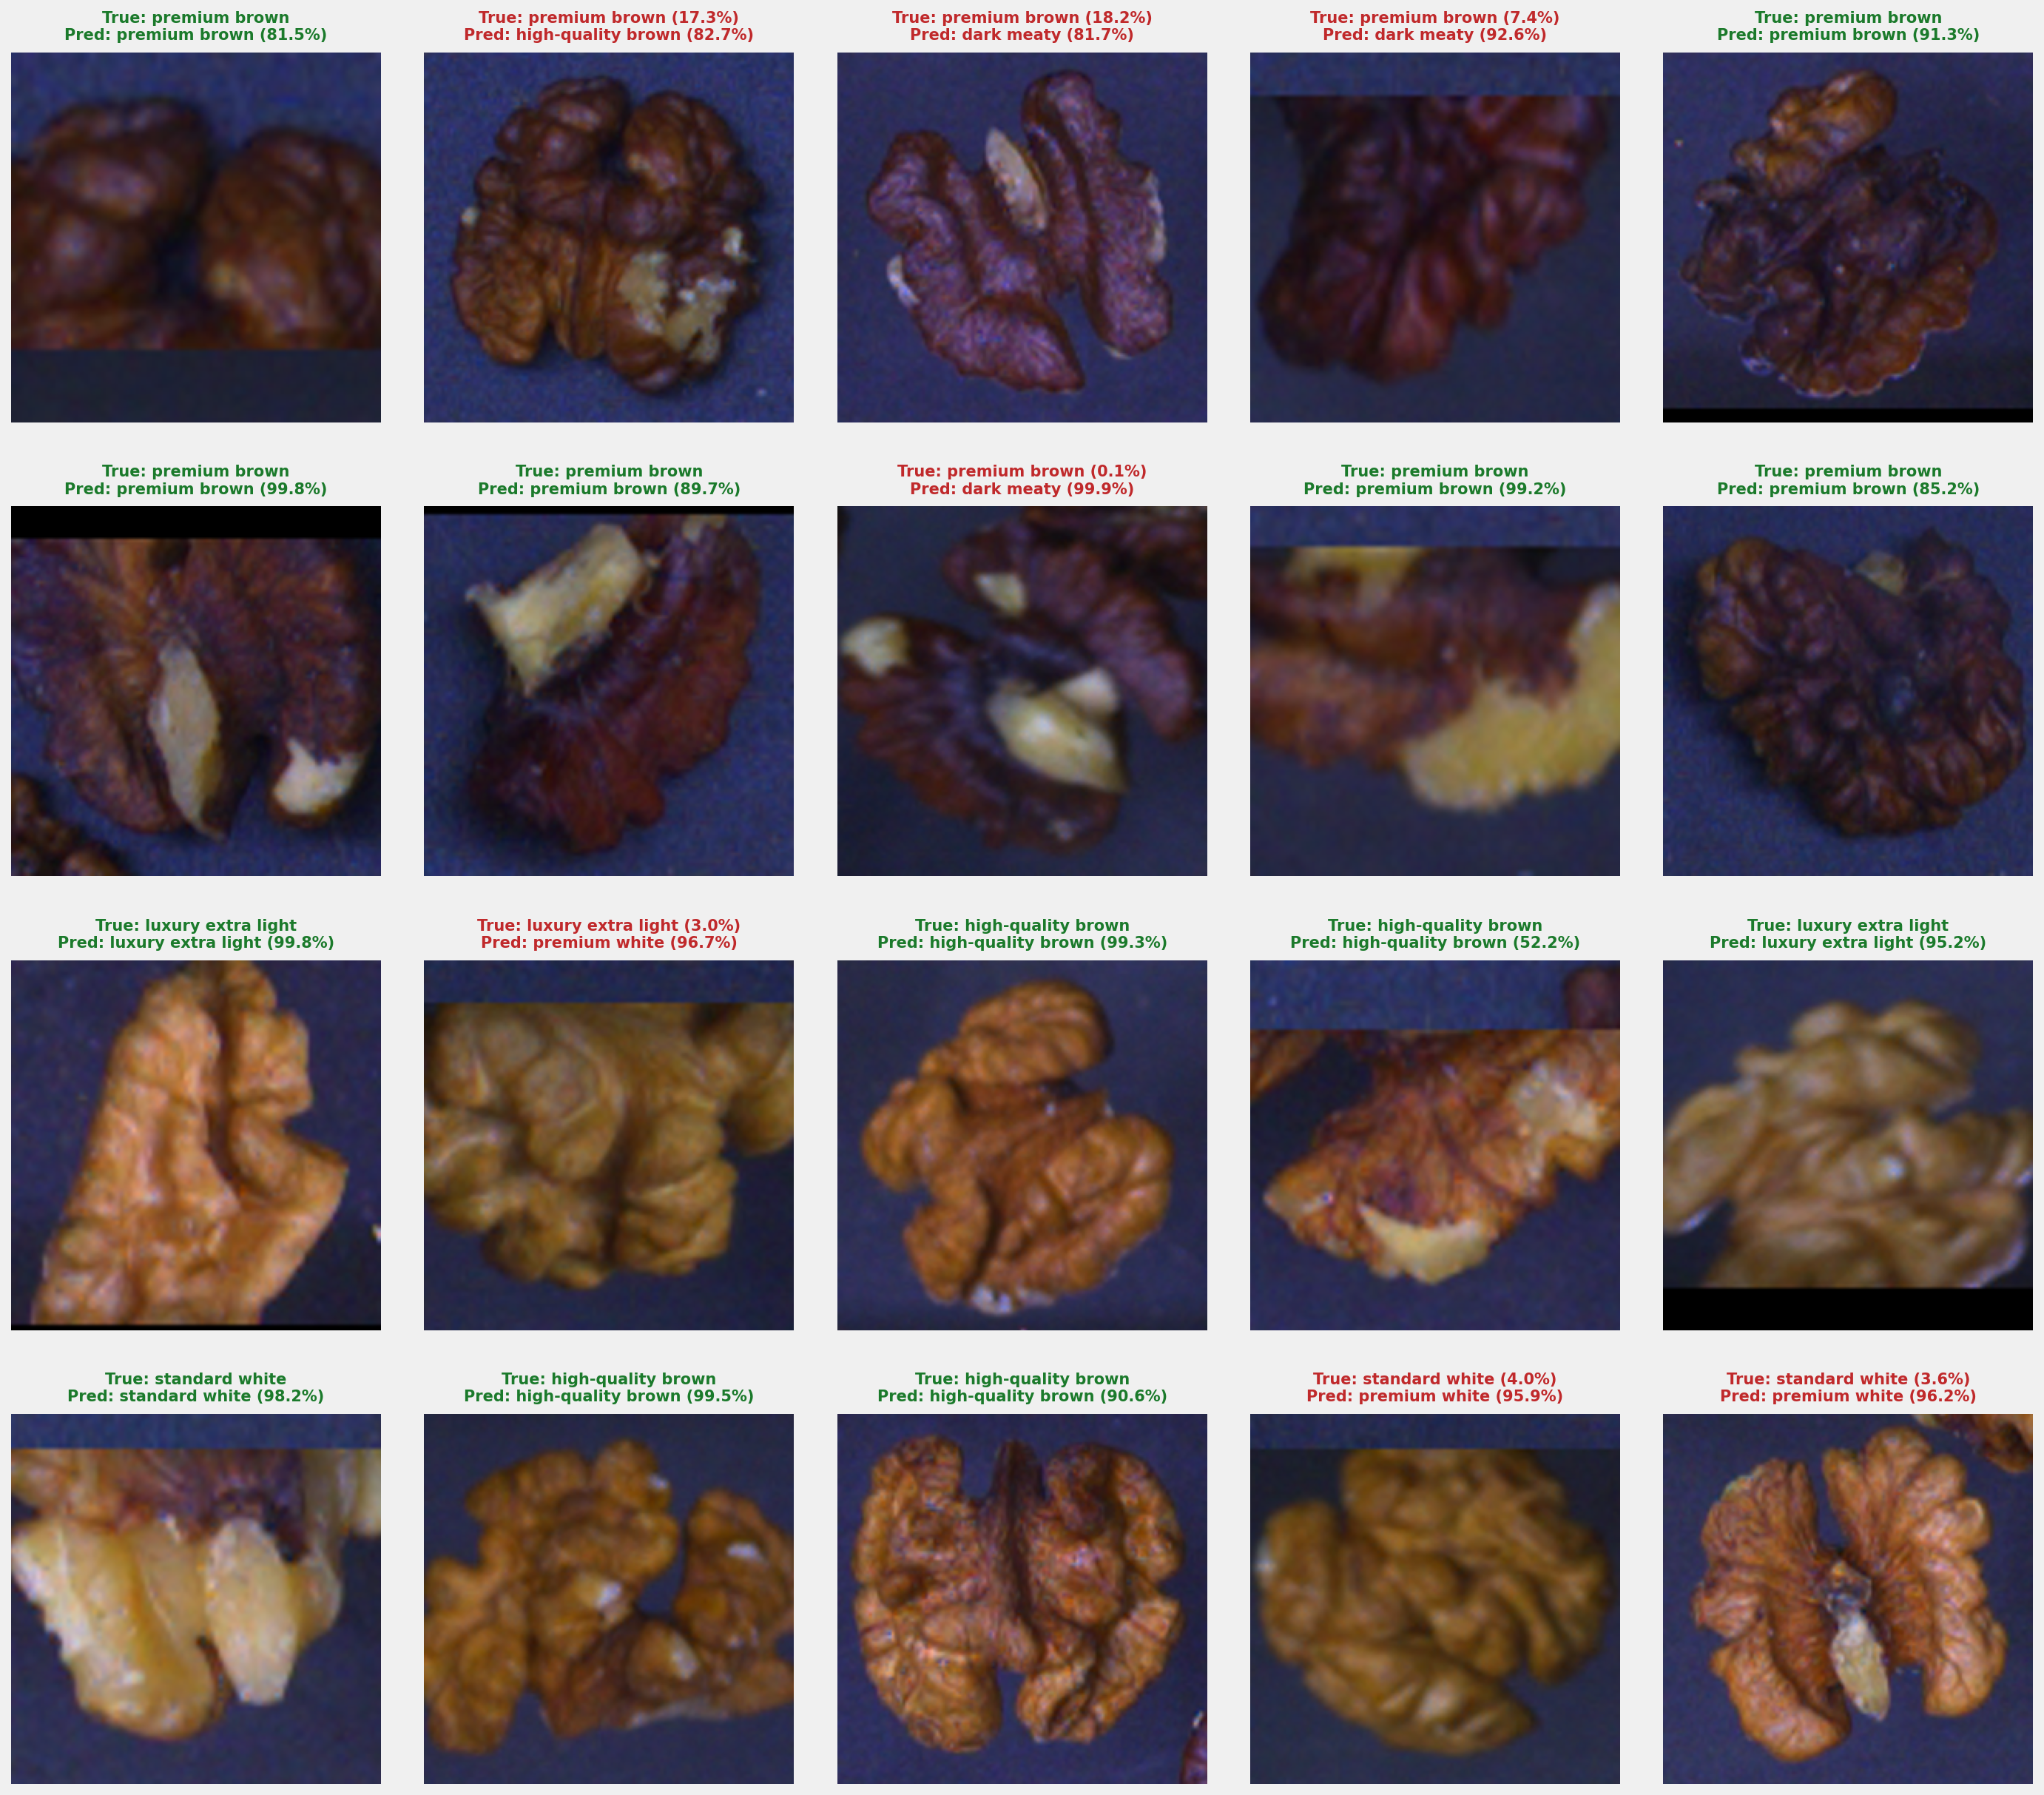
\includegraphics[width=\textwidth]{figures/16shot_baseline_preds.png}
        \caption{Plain LoRA}
    \end{subfigure}
    \hfill
    \begin{subfigure}[b]{0.235\textwidth}
        \includegraphics[width=\textwidth]{figures2/run1_baseline_16shot_test_preds.png}
        \caption{Run 1 --- Baseline}
    \end{subfigure}
    \hfill
    \begin{subfigure}[b]{0.235\textwidth}
        \includegraphics[width=\textwidth]{figures2/run2_learnable_tokens_16shot_test_preds.png}
        \caption{Run 2 --- + Cls Tokens}
    \end{subfigure}
    \hfill
    \begin{subfigure}[b]{0.235\textwidth}
        \includegraphics[width=\textwidth]{figures2/run3_ordinal_loss_16shot_test_preds.png}
        \caption{Run 3 --- + Ordinal}
    \end{subfigure}

    \vspace{4pt}

    \begin{subfigure}[b]{0.235\textwidth}
        \includegraphics[width=\textwidth]{figures2/run4_promptsrc_16shot_test_preds.png}
        \caption{Run 4 --- + PromptSRC}
    \end{subfigure}
    \hfill
    \begin{subfigure}[b]{0.235\textwidth}
        \includegraphics[width=\textwidth]{figures2/run5_full_method_16shot_test_preds.png}
        \caption{Run 5 --- + Full Method}
    \end{subfigure}
    \hfill
    \begin{subfigure}[b]{0.235\textwidth}
        \includegraphics[width=\textwidth]{figures2/run6_rt_lora_16shot_test_preds.png}
        \caption{Run 6 --- RT-LoRA}
    \end{subfigure}
    \hfill
    \begin{subfigure}[b]{0.235\textwidth}
        \includegraphics[width=\textwidth]{figures2/run7_csc_vision_16shot_test_preds.png}
        \caption{Run 7 --- CSC Vision}
    \end{subfigure}

    \vspace{4pt}

    \begin{subfigure}[b]{0.235\textwidth}
        \includegraphics[width=\textwidth]{figures2/run8_csc_both_16shot_test_preds.png}
        \caption{Run 8 --- CSC Dual}
    \end{subfigure}
    \hfill
    \begin{subfigure}[b]{0.235\textwidth}
        \includegraphics[width=\textwidth]{figures2/run9_staged_csc_vision_16shot_test_preds.png}
        \caption{Run 9 --- CSC100 Vision}
    \end{subfigure}
    \hfill
    \begin{subfigure}[b]{0.235\textwidth}
        \includegraphics[width=\textwidth]{figures2/run10_staged_csc_both_16shot_test_preds.png}
        \caption{Run 10 --- CSC100 Dual}
    \end{subfigure}
    \hfill
    \begin{subfigure}[b]{0.235\textwidth}
        \centering
        \vspace{0.8cm}
        \textit{\scriptsize [11 Evaluated Models]}
    \end{subfigure}

    \caption{Sample test-set predictions at 16-shot across all 11 models.}
    \label{fig:sample_preds_16shot}
\end{figure}

\subsection{Attention Maps via EigenCAM}

\begin{figure}[H]
    \centering
    \begin{subfigure}[b]{0.235\textwidth}
        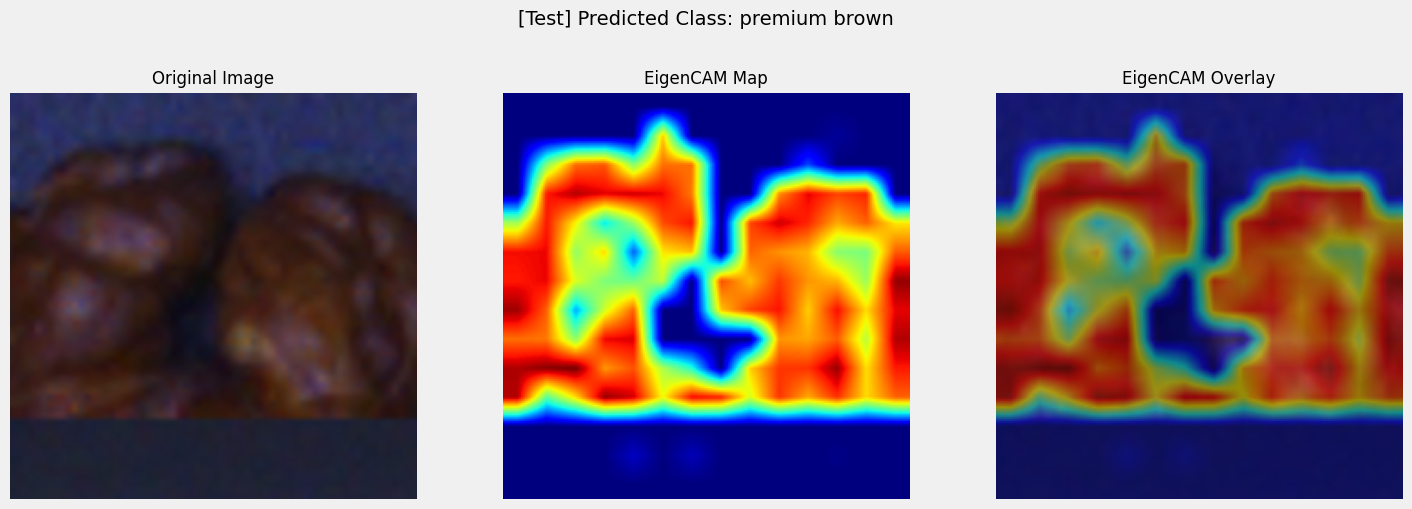
\includegraphics[width=\textwidth]{figures/16shot_baseline_attn_img0.png}
        \caption{Plain CLIP-LoRA}
    \end{subfigure}
    \hfill
    \begin{subfigure}[b]{0.235\textwidth}
        \includegraphics[width=\textwidth]{figures2/run1_baseline_16shot_attn2.png}
        \caption{Run 1 --- Baseline}
    \end{subfigure}
    \hfill
    \begin{subfigure}[b]{0.235\textwidth}
        \includegraphics[width=\textwidth]{figures2/run2_learnable_tokens_16shot_attn2.png}
        \caption{Run 2 --- + Cls Tokens}
    \end{subfigure}
    \hfill
    \begin{subfigure}[b]{0.235\textwidth}
        \includegraphics[width=\textwidth]{figures2/run3_ordinal_loss_16shot_attn2.png}
        \caption{Run 3 --- + Ordinal}
    \end{subfigure}

    \vspace{4pt}

    \begin{subfigure}[b]{0.235\textwidth}
        \includegraphics[width=\textwidth]{figures2/run4_promptsrc_16shot_attn2.png}
        \caption{Run 4 --- + PromptSRC}
    \end{subfigure}
    \hfill
    \begin{subfigure}[b]{0.235\textwidth}
        \includegraphics[width=\textwidth]{figures2/run5_full_method_16shot_attn2.png}
        \caption{Run 5 --- + Full Method}
    \end{subfigure}
    \hfill
    \begin{subfigure}[b]{0.235\textwidth}
        \includegraphics[width=\textwidth]{figures2/run6_rt_lora_16shot_attn2.png}
        \caption{Run 6 --- RT-LoRA}
    \end{subfigure}
    \hfill
    \begin{subfigure}[b]{0.235\textwidth}
        \includegraphics[width=\textwidth]{figures2/run7_csc_vision_16shot_attn2.png}
        \caption{Run 7 --- CSC Vision}
    \end{subfigure}

    \vspace{4pt}

    \begin{subfigure}[b]{0.235\textwidth}
        \includegraphics[width=\textwidth]{figures2/run8_csc_both_16shot_attn2.png}
        \caption{Run 8 --- CSC Dual}
    \end{subfigure}
    \hfill
    \begin{subfigure}[b]{0.235\textwidth}
        \includegraphics[width=\textwidth]{figures2/run9_staged_csc_vision_16shot_attn2.png}
        \caption{Run 9 --- CSC100 Vision}
    \end{subfigure}
    \hfill
    \begin{subfigure}[b]{0.235\textwidth}
        \includegraphics[width=\textwidth]{figures2/run10_staged_csc_both_16shot_attn2.png}
        \caption{Run 10 --- CSC100 Dual}
    \end{subfigure}
    \hfill
    \begin{subfigure}[b]{0.235\textwidth}
        \centering
        \vspace{0.8cm}
        \textit{\scriptsize [11 Evaluated Models]}
    \end{subfigure}

    \caption{EigenCAM attention maps at 16-shot across all 11 models.}
    \label{fig:attention_maps_16shot}
\end{figure}

\subsection{Attention Map Progression Across Shots}

\begin{figure}[H]
    \centering
    \includegraphics[height=0.72\textheight,keepaspectratio]{figures2/comparison_attention_progression.png}
    \caption{Attention map progression across 1-shot, 4-shot, 16-shot, and 32-shot counts across all 11 models.}
    \label{fig:attention_progression_all}
\end{figure}

\end{document}
